\subsection{Controller}
%
%\begin{frame}{Controller}{}
%
%  \begin{block}{PID}
%
%  \end{block}
%  
%  \begin{block}{Tunning}
%
%  \end{block}
%
%  \begin{block}{Comparion}
%
%  \end{block}
%
%\end{frame}

%Overview
\begin{frame}{Modelling}{Moving Angle System}
  \begin{block}{Moving Angle System:}

	  \begin{itemize}
	  	\item Sensor
	  	\item Servomotor
	  	\item Gear
	  	\item Controller
	  \end{itemize}

	  \begin{figure}
        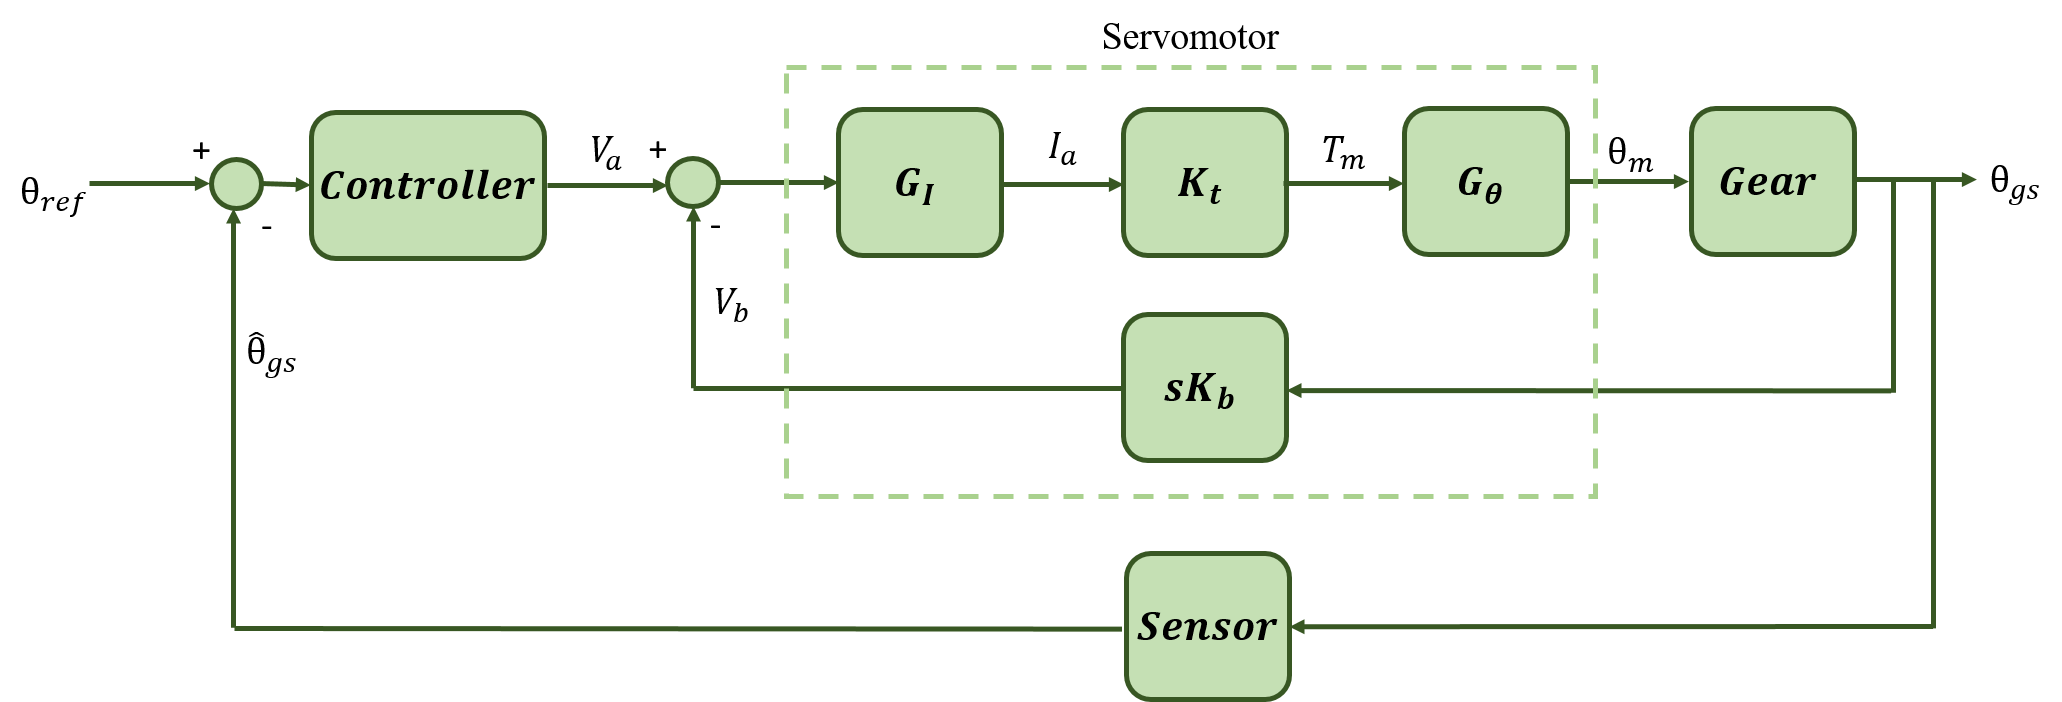
\includegraphics[scale=0.26]{../report/figures/servo+gear+noise.png}
      \end{figure}
  
  \end{block}
\end{frame}

%Sensor
\begin{frame}{Modelling}{Moving Angle System}
  \begin{block}{Moving Angle System:}

	  \begin{itemize}
	  	\item Sensor
	  \end{itemize}

	  \begin{figure}
        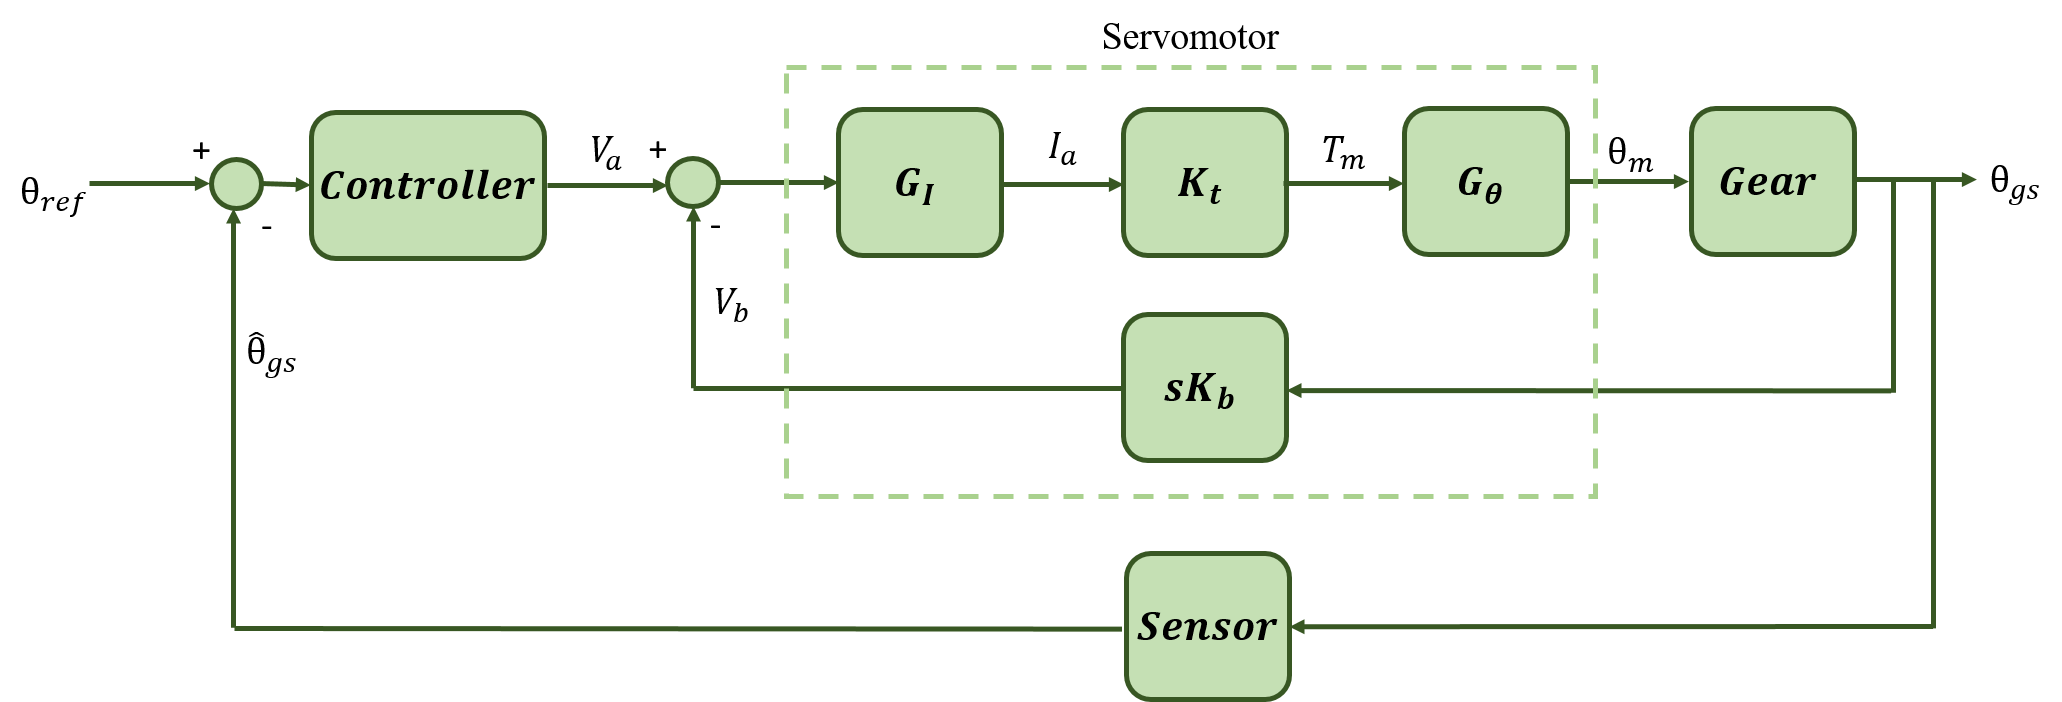
\includegraphics[scale=0.26]{../report/figures/servo+gear+noise.png}
      \end{figure}
  
  \end{block}
\end{frame}

%Servomotor
\begin{frame}{Modelling}{Moving Angle System}
  \begin{block}{Moving Angle System:}

	  \begin{itemize}
	  	\item Servomotor
	  \end{itemize}

	  \begin{figure}
        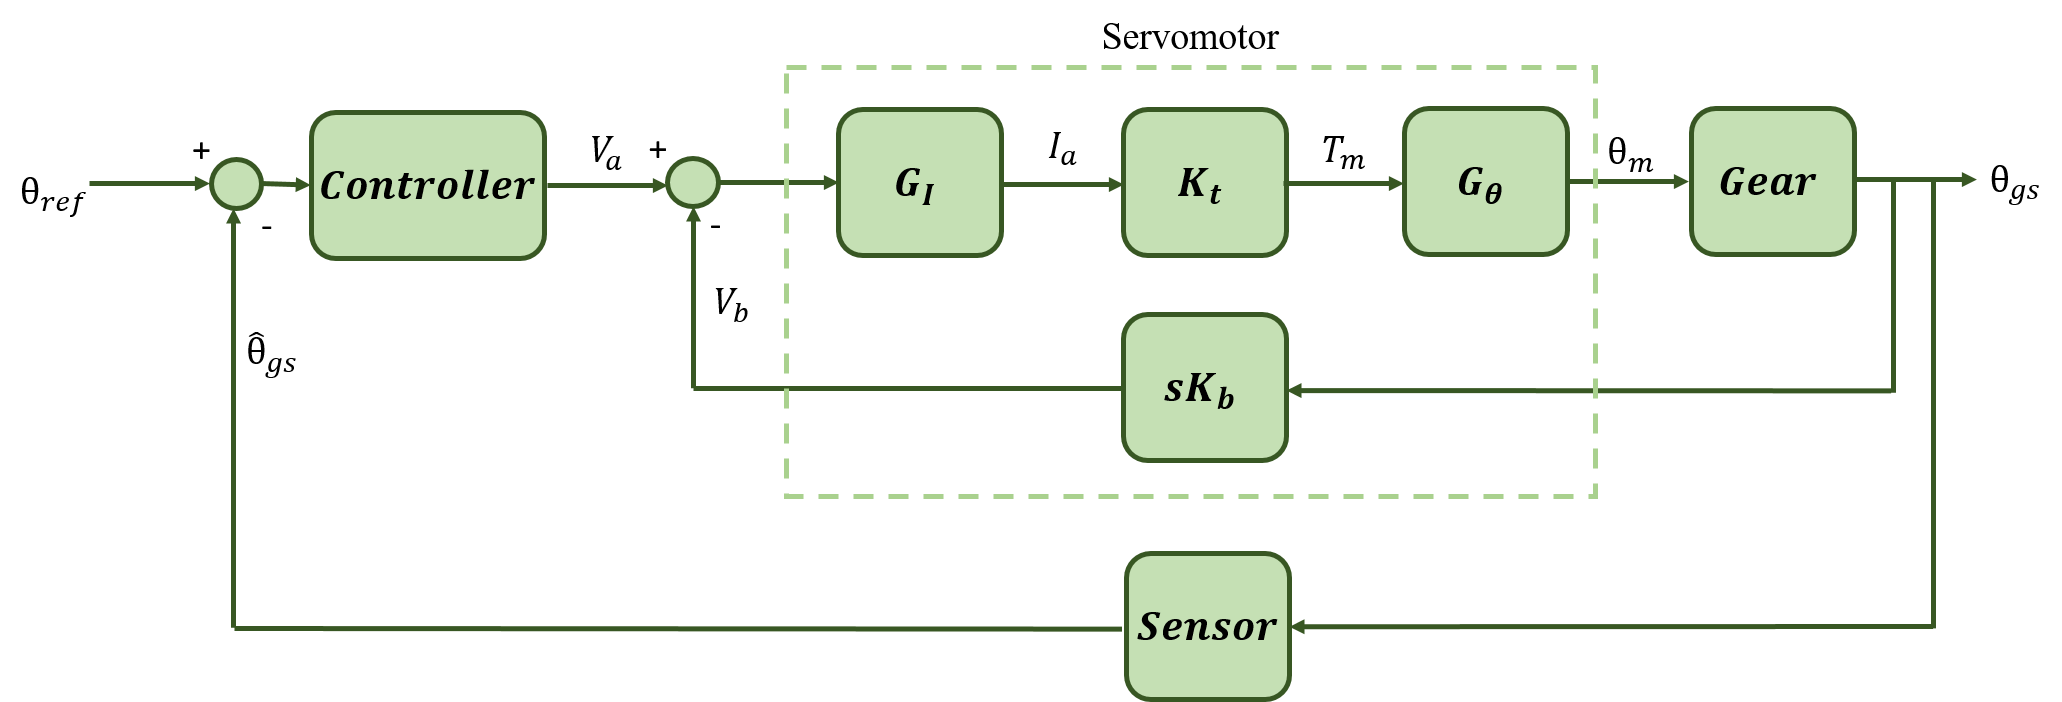
\includegraphics[scale=0.26]{../report/figures/servo+gear+noise.png}
      \end{figure}
  
  \end{block}
\end{frame}

%Gear
\begin{frame}{Modelling}{Moving Angle System}
  \begin{block}{Moving Angle System:}

	  \begin{itemize}
	  	\item Gear
	  \end{itemize}

	  \begin{figure}
        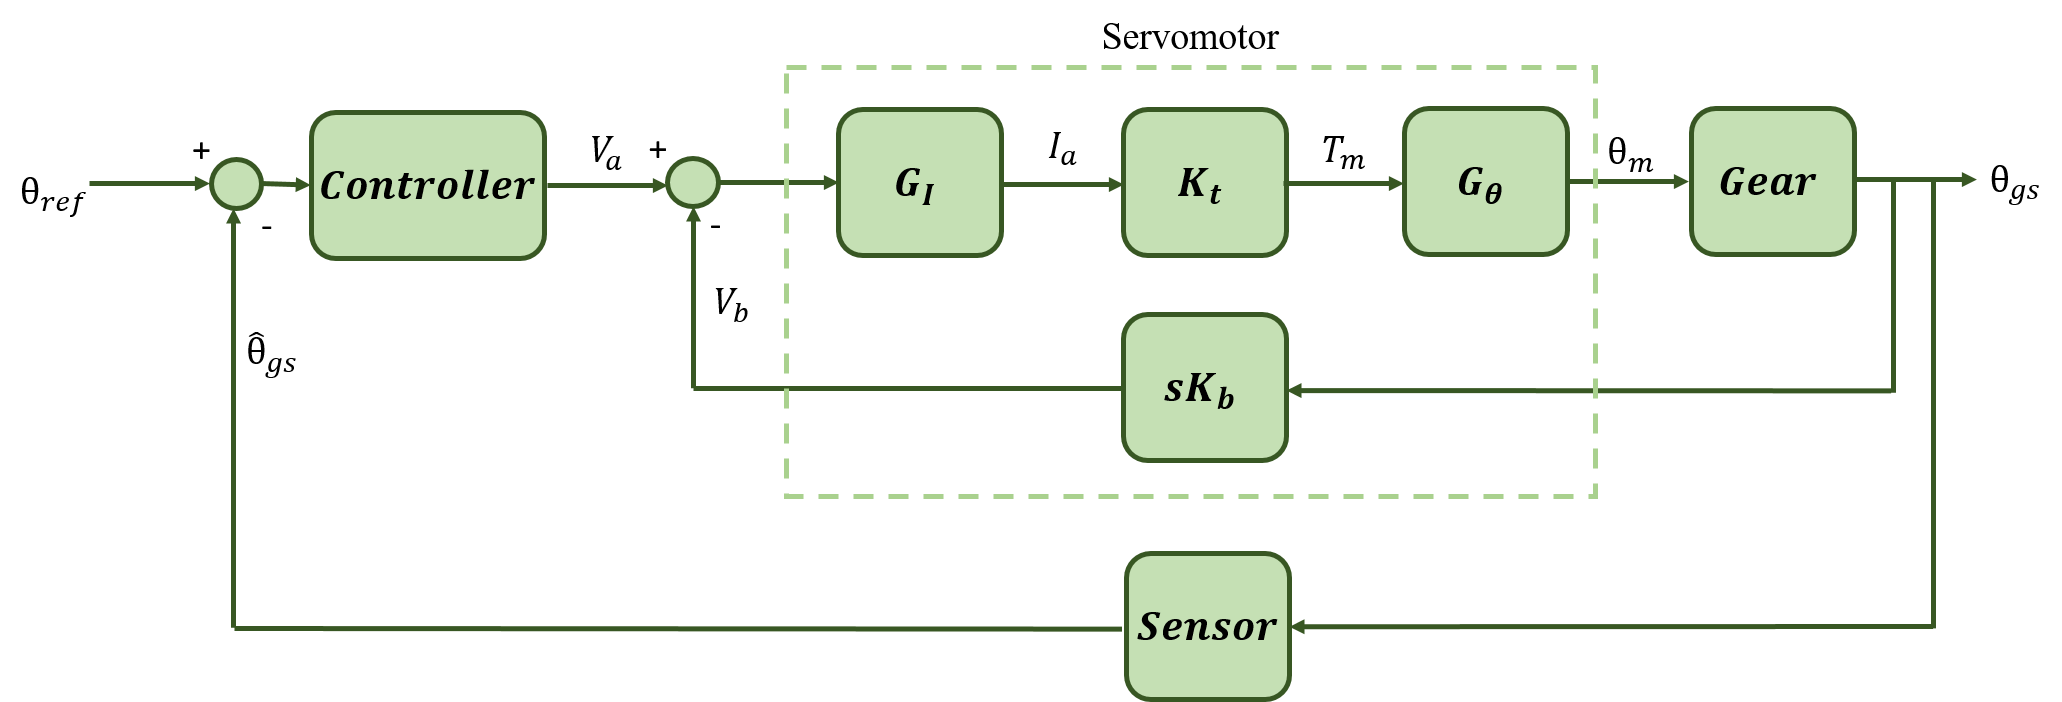
\includegraphics[scale=0.26]{../report/figures/servo+gear+noise.png}
      \end{figure}
  
  \end{block}
\end{frame}

%Controller
\begin{frame}{Modelling}{Moving Angle System}
  \begin{block}{Moving Angle System:}

	  \begin{itemize}
	  	\item Controller
	  \end{itemize}

	  \begin{figure}
        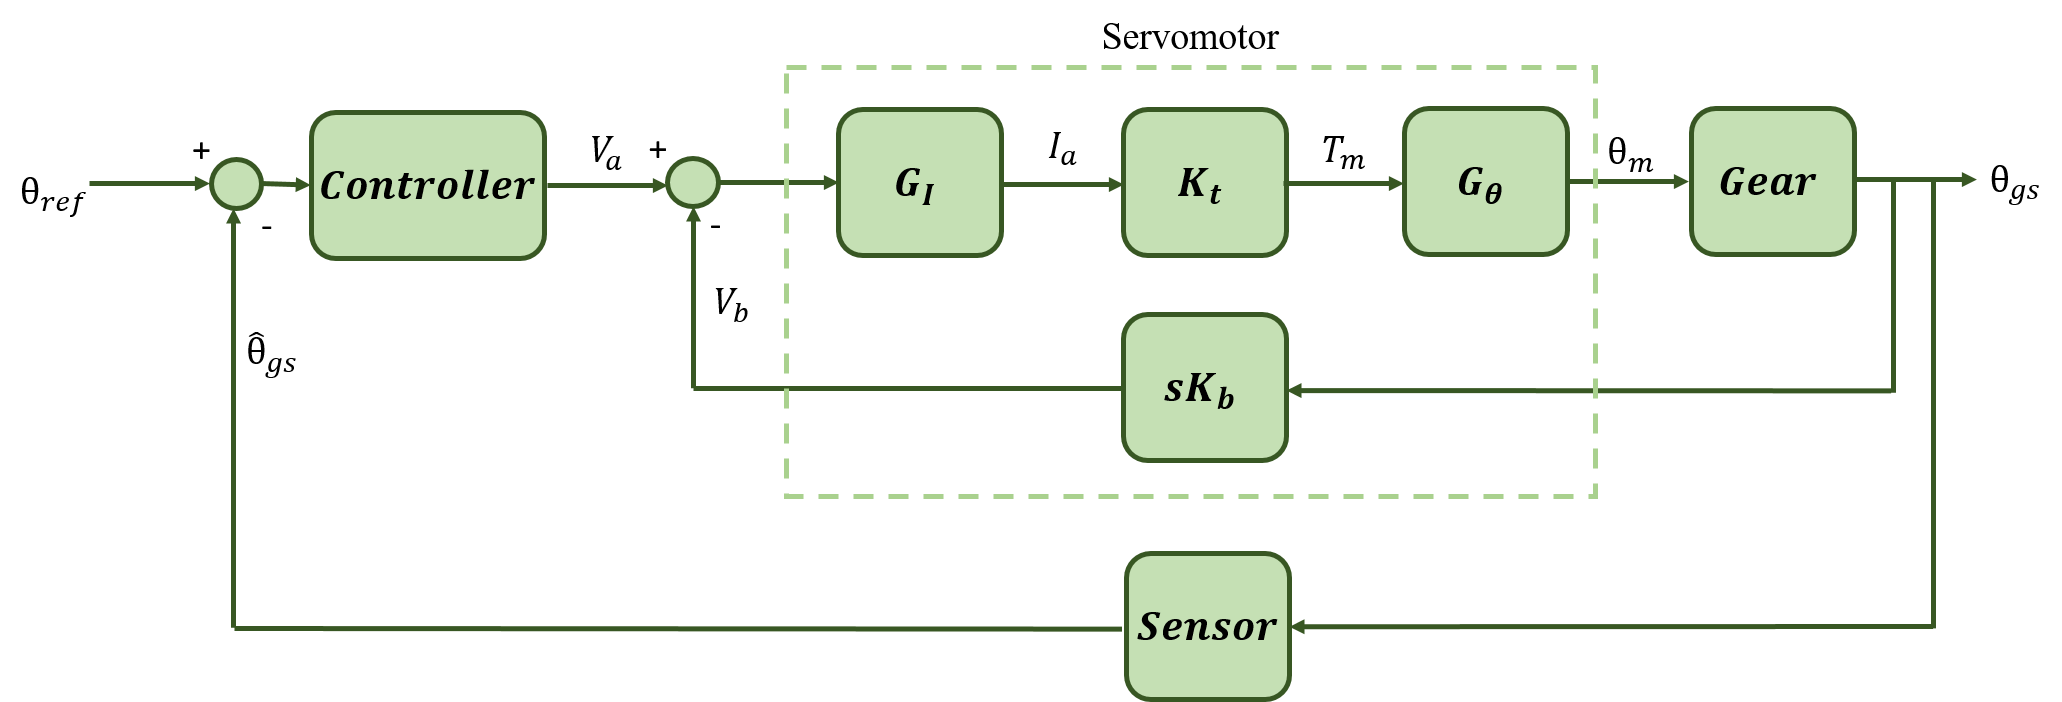
\includegraphics[scale=0.26]{../report/figures/servo+gear+noise.png}
      \end{figure}
  
  \end{block}
\end{frame}

%%% CONTROLLER


%Controller
\begin{frame}{Controller}{Different controllers}
  \begin{block}{Different controllers:}

	  \begin{itemize}
	  	\item PID Theory
	  \end{itemize}


  
  \end{block}
\end{frame}

%Controller P
\begin{frame}{Controller}{Different controllers}
  \begin{block}{P Controller}

	  \begin{itemize}
	  	\item Output always proportional to the error
	  \end{itemize}

	  \begin{figure}
        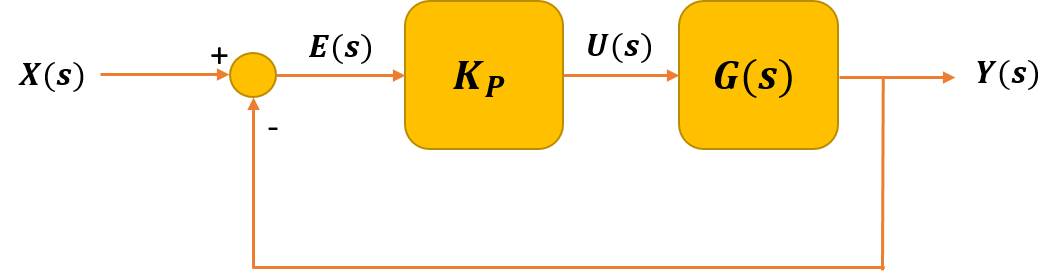
\includegraphics[scale=0.26]{../report/figures/propor_controller.png}
      \end{figure}
  
  \end{block}
\end{frame}

%Controller I
\begin{frame}{Controller}{Different controllers}
  \begin{block}{I Controller}

	  \begin{itemize}
	  	\item Sums the error term over time
	  	\item Tends the steady state error to zero
	  	\item Cause the present value to overshoot the reference value
	  \end{itemize}

	  \begin{figure}
        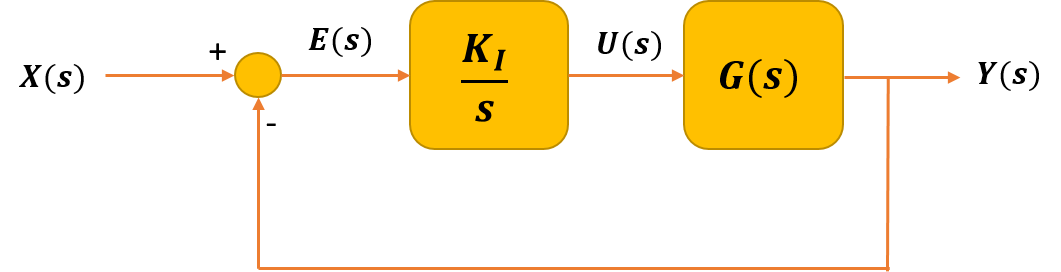
\includegraphics[scale=0.26]{../report/figures/integ_controller.png}
      \end{figure}
  
  \end{block}
\end{frame}

%Controller D
\begin{frame}{Controller}{Different controllers}
  \begin{block}{D Controller}

	  \begin{itemize}
	  	\item Acts as a brake on the control effort
	  	\item Highly sensitive to noise
	  \end{itemize}

	  \begin{figure}
        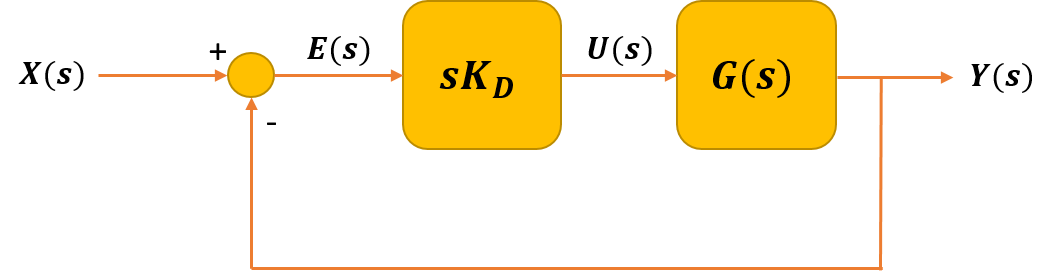
\includegraphics[scale=0.26]{../report/figures/deriv_controller.png}
      \end{figure}
  
  \end{block}
\end{frame}

%Controller PI
\begin{frame}{Controller}{Different controllers}
  \begin{block}{PI Controller}

	  \begin{itemize}
	  	\item Mainly to eliminate the steady state error
	  	\item Negative impact in the speed of the response
	  	\item This controller should be applied when speed is not an important parameter
	  \end{itemize}

	  \begin{figure}
        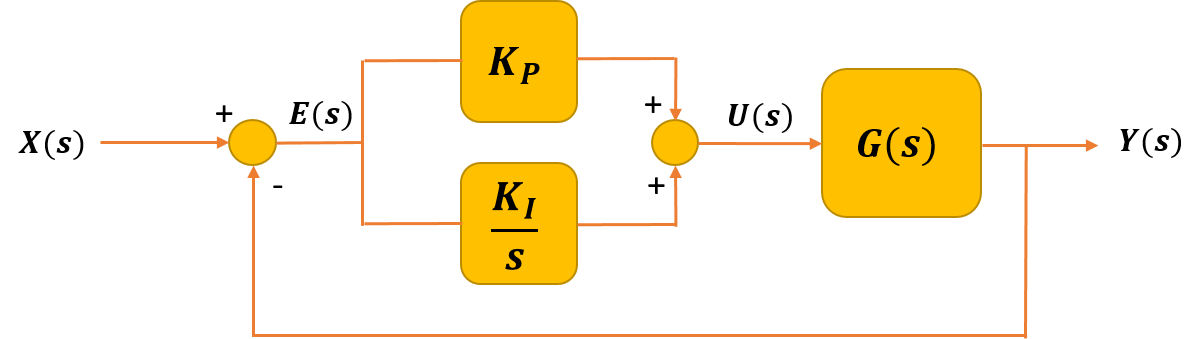
\includegraphics[scale=0.26]{../report/figures/PI_controller.png}
      \end{figure}
  
  \end{block}
\end{frame}


%Controller PD
\begin{frame}{Controller}{Different controllers}
  \begin{block}{PD Controller}

	  \begin{itemize}
	  	\item Why is PD alone good?
	  \end{itemize}

	  \begin{figure}
        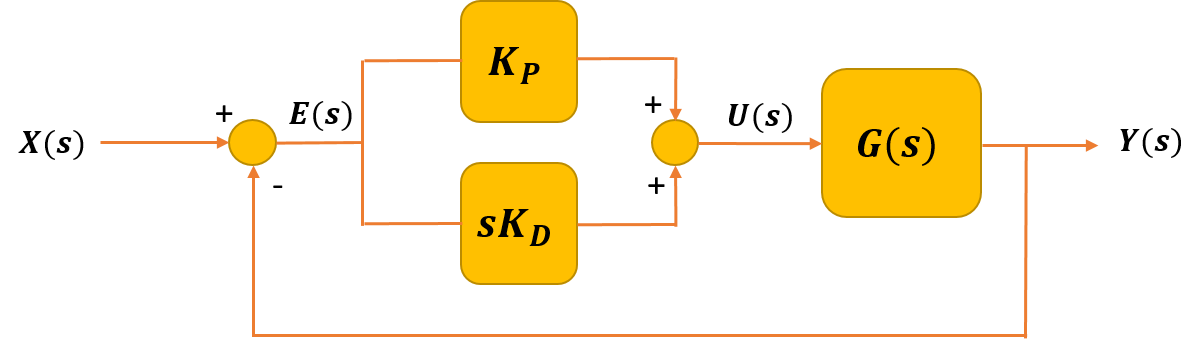
\includegraphics[scale=0.26]{../report/figures/PD_controller.png}
      \end{figure}
  
  \end{block}
\end{frame}

%Controller PID
\begin{frame}{Controller}{Different controllers}
  \begin{block}{PID Controller}

	  \begin{itemize}
	  	\item Zero steady state error
	  	\item Fast response
	  	\item Higher stability
	  \end{itemize}

	  \begin{figure}
        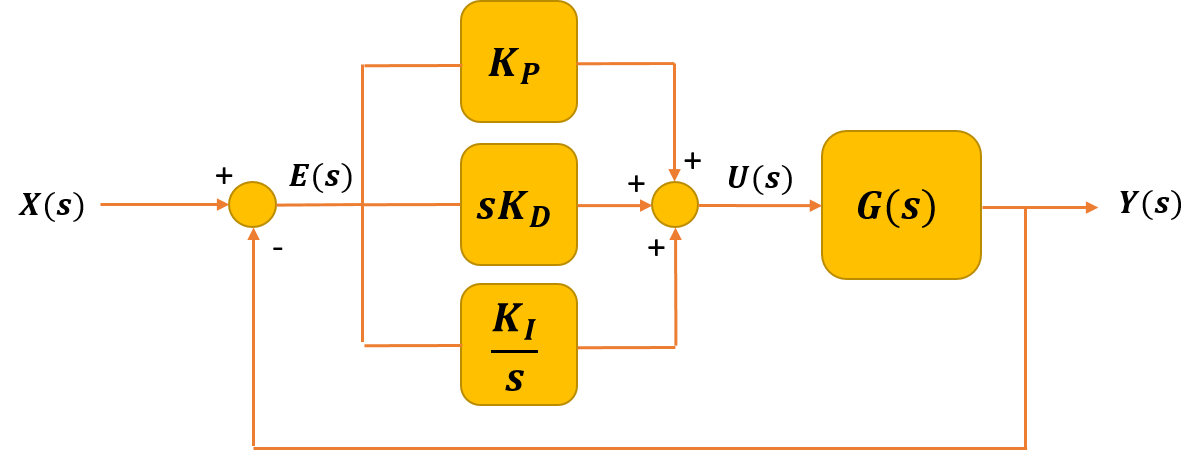
\includegraphics[scale=0.26]{../report/figures/PID_controller.png}
      \end{figure}
  
  \end{block}
\end{frame}

%Tuning Method
\begin{frame}{Controller}{Tuning Methods}
  \begin{block}{Good Gain Method}

%	  \begin{figure}
%        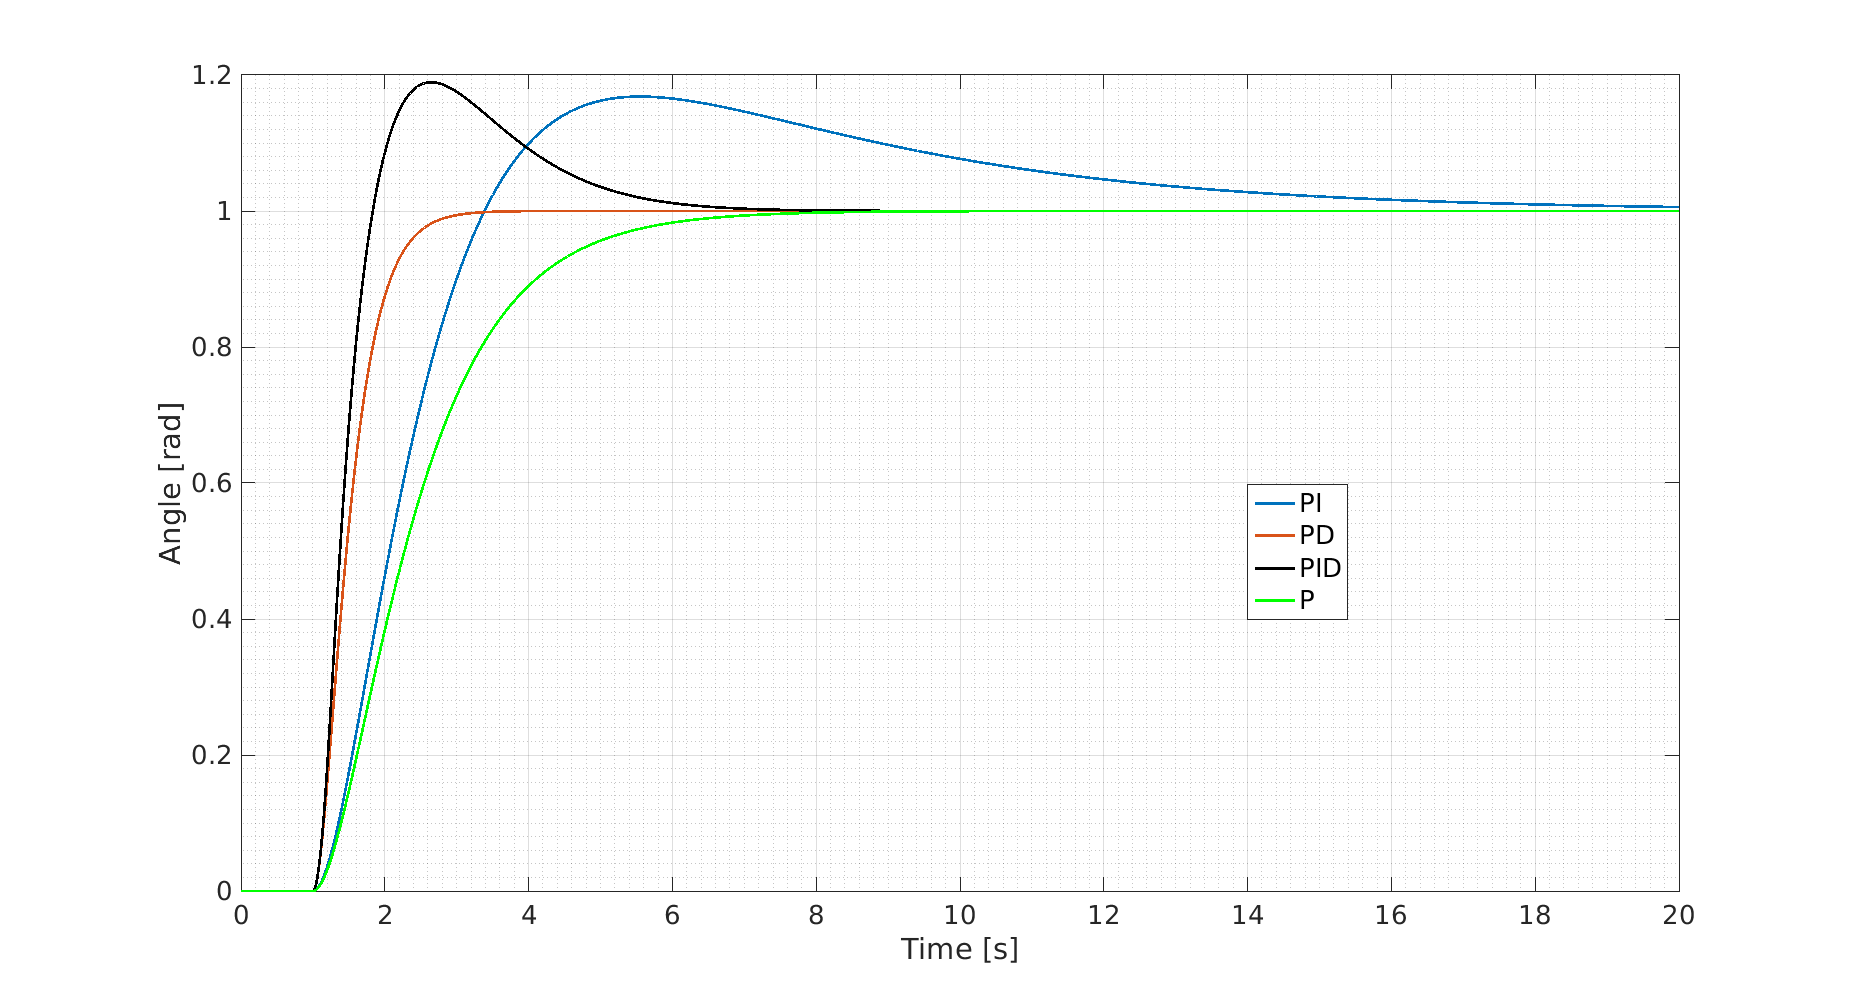
\includegraphics[scale=0.20]{../report/figures/full_comp.png}
%      \end{figure}
  
  \end{block}
\end{frame}

%Tuning Method
\begin{frame}{Controller}{Tuning Methods}
  \begin{block}{PID Simulink Box}

%	  \begin{figure}
%        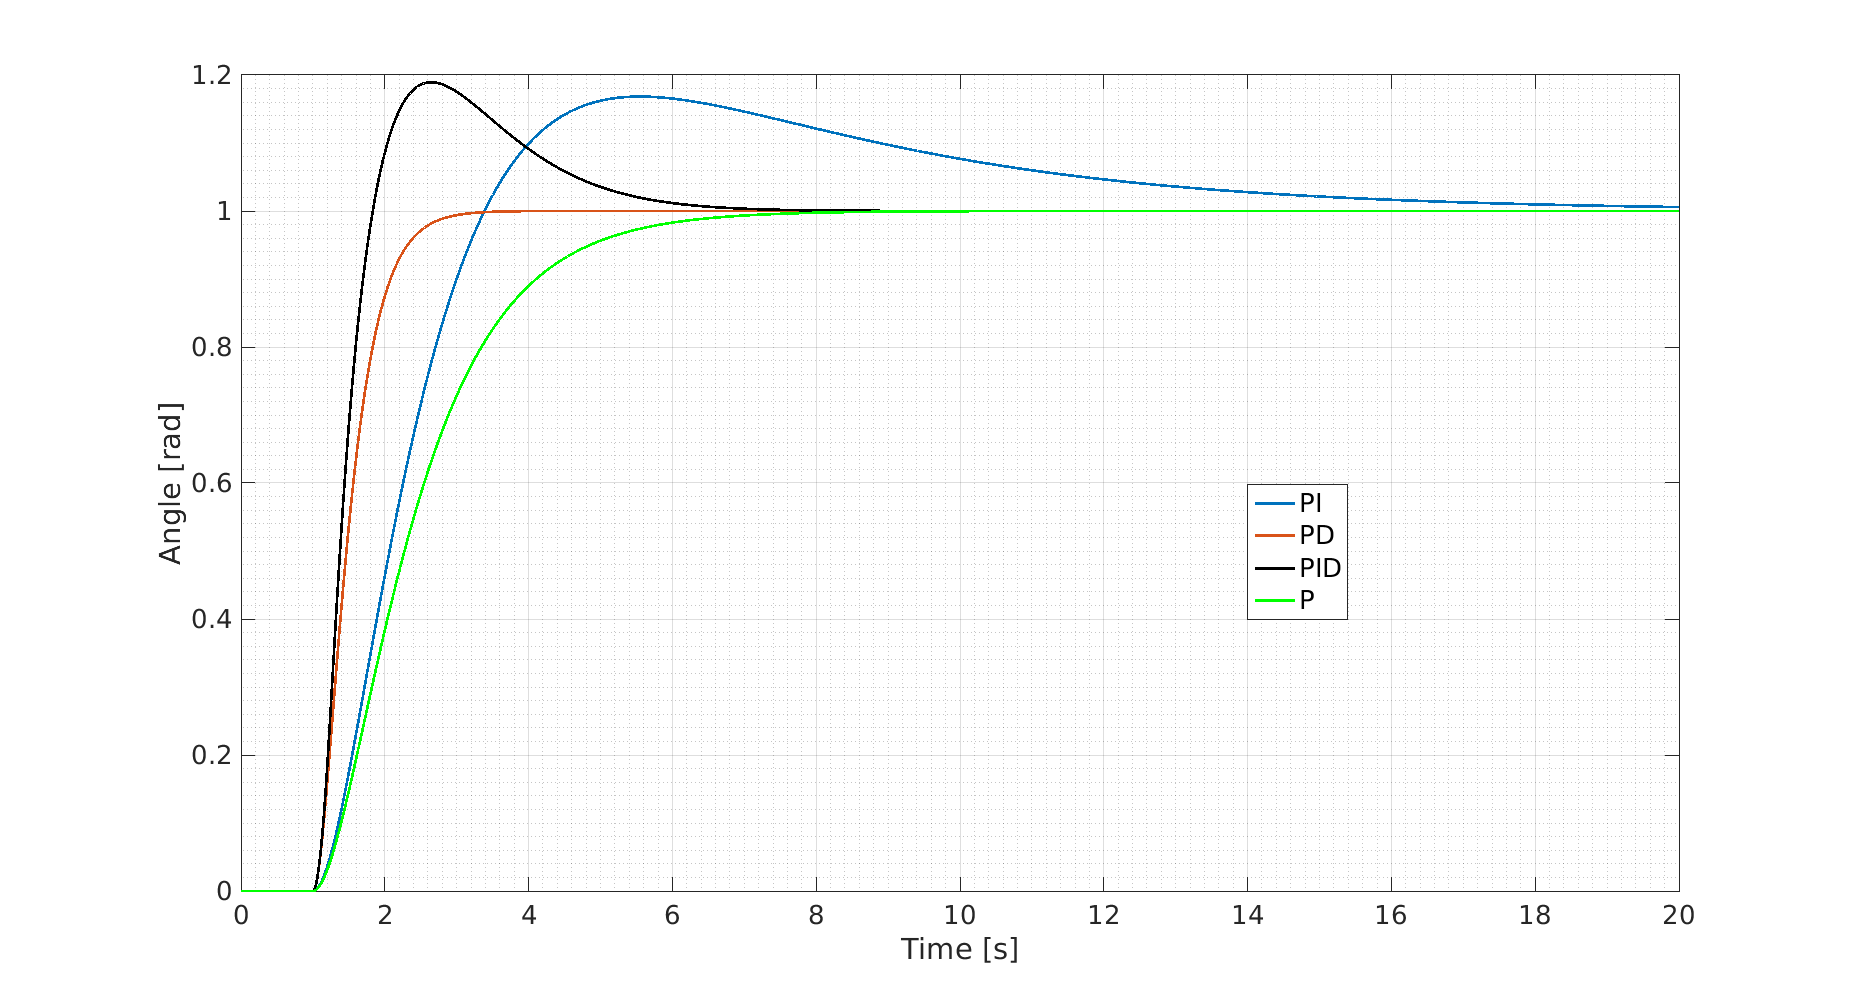
\includegraphics[scale=0.20]{../report/figures/full_comp.png}
%      \end{figure}
  
  \end{block}
\end{frame}

%Comparison
\begin{frame}{Controller}{Comparison of step responses}
  \begin{block}{Different controllers without noise:}

	  \begin{figure}
        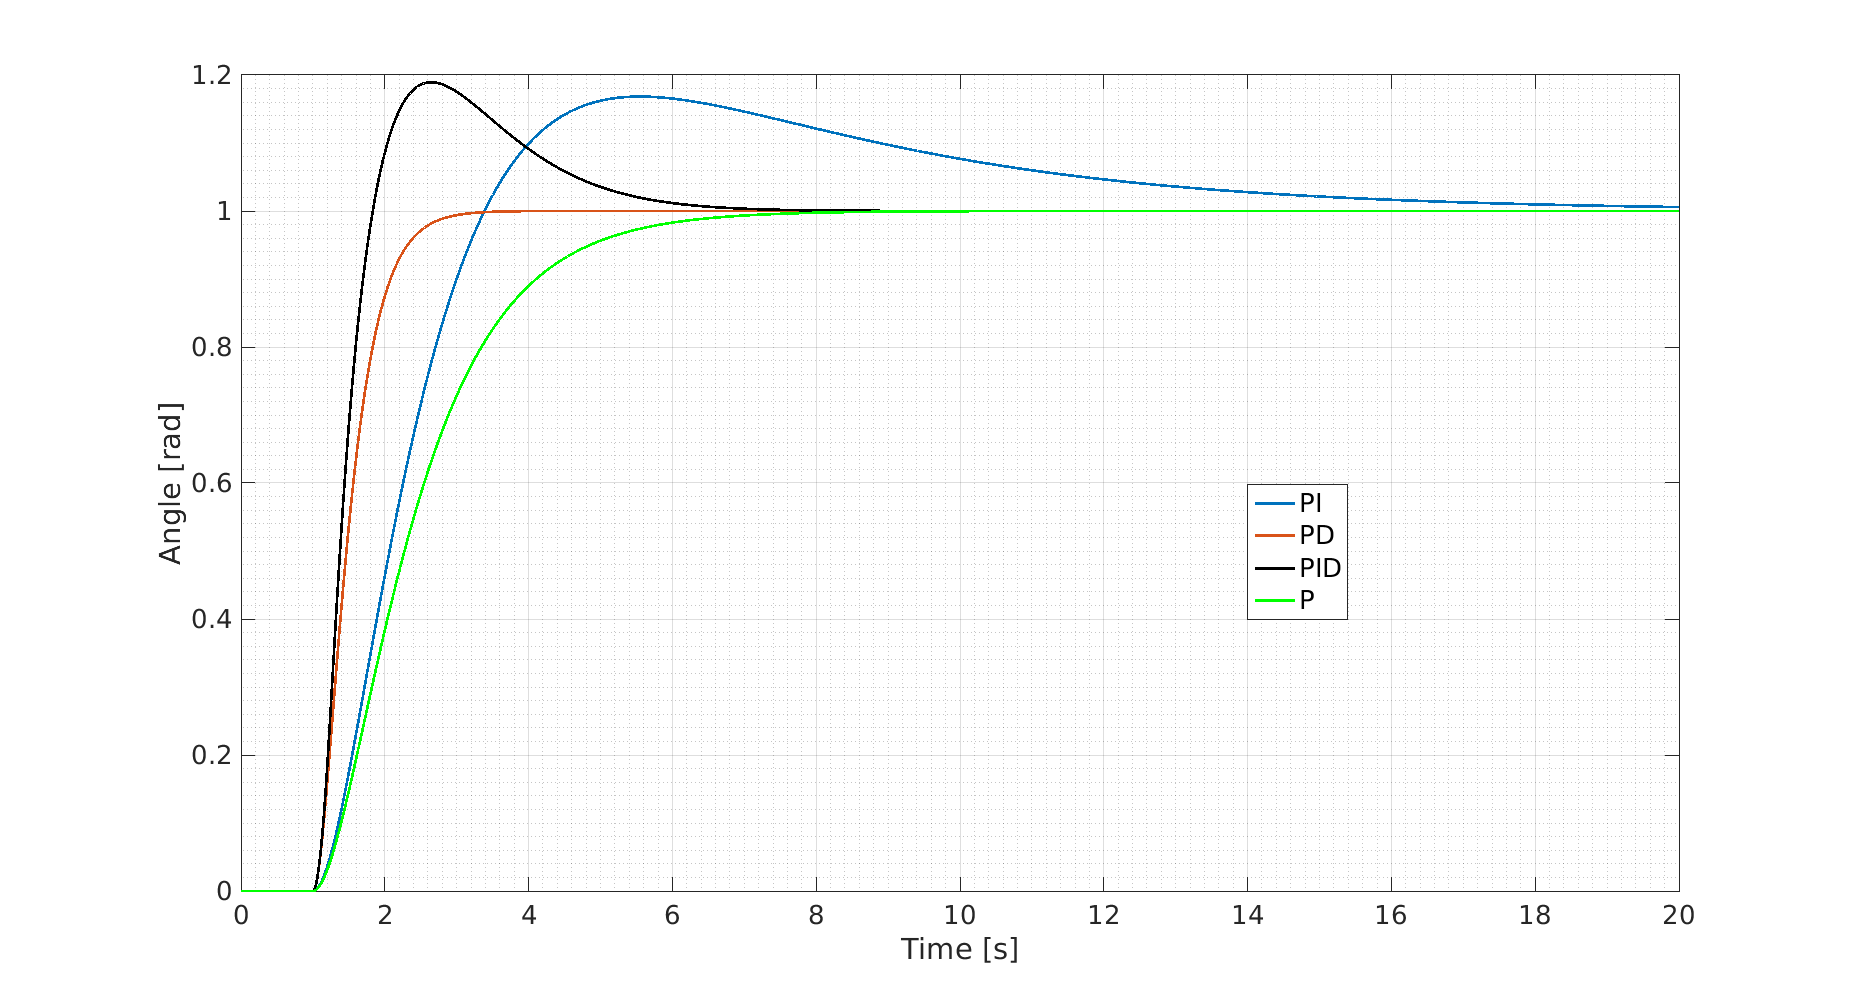
\includegraphics[scale=0.20]{../report/figures/full_comp.png}
      \end{figure}
  
  \end{block}
\end{frame}

%Comparison
\begin{frame}{Controller}{Comparison of step responses}
  \begin{block}{Different controllers with noise:}

	  \begin{figure}
        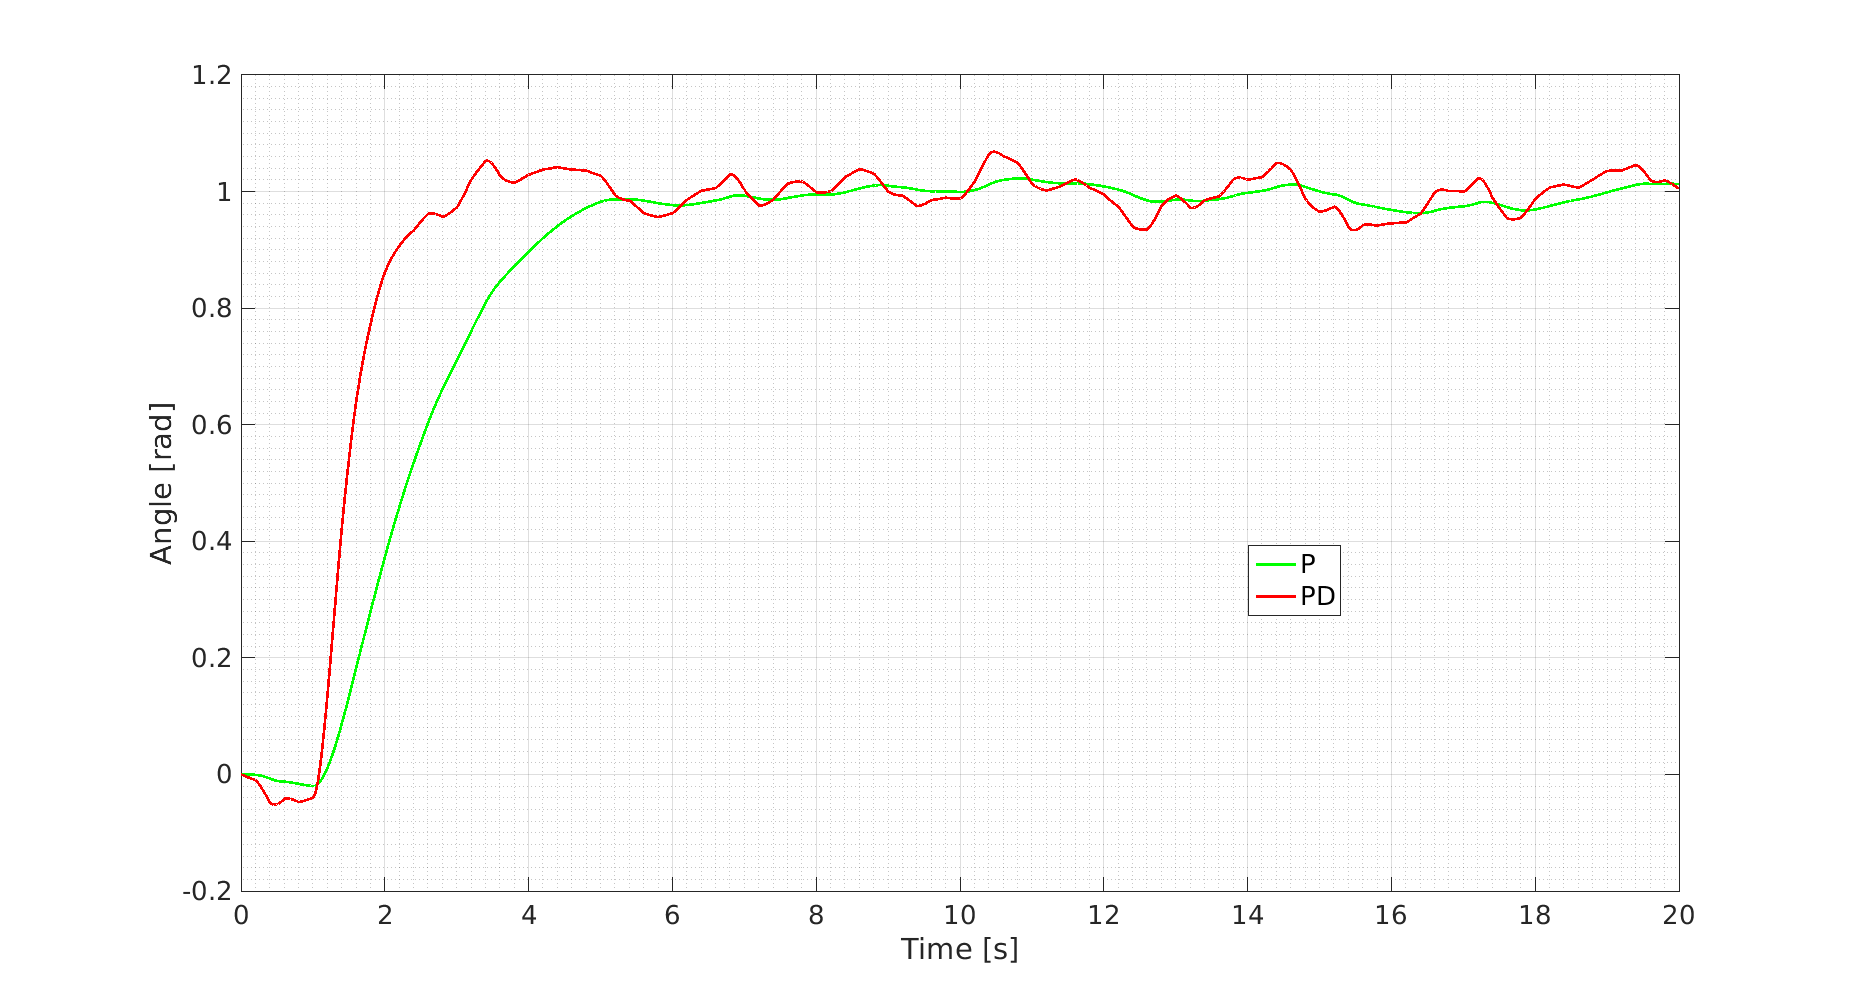
\includegraphics[scale=0.20]{../report/figures/PD_noise.png}
      \end{figure}
  
  \end{block}
\end{frame}

